\documentclass[12pt, a4paper]{article}

\usepackage[czech]{babel}
\usepackage{lmodern}
\usepackage[utf8]{inputenc}
\usepackage[T1]{fontenc}
\usepackage{graphicx}
\usepackage{amsmath}
\usepackage[hidelinks,unicode]{hyperref}
\usepackage{float}
\usepackage{listings}
\usepackage{tikz}
\usepackage{xcolor}
\usepackage[final]{pdfpages}
\usepackage{tabularx}

\definecolor{mauve}{rgb}{0.58,0,0.82}
\usetikzlibrary{shapes,positioning,matrix,arrows}

\newcommand{\img}[1]{(viz obr. \ref{#1})}

\definecolor{pblue}{rgb}{0.13,0.13,1}
\definecolor{pgreen}{rgb}{0,0.5,0}
\definecolor{pred}{rgb}{0.9,0,0}
\definecolor{pgrey}{rgb}{0.46,0.45,0.48}

\lstset{frame=tb,
  language=C,
  aboveskip=3mm,
  belowskip=3mm,
  showstringspaces=false,
  columns=flexible,
  basicstyle={\small\ttfamily},
  numbers=none,
  numberstyle=\tiny\color{gray},
  keywordstyle=\color{blue},
  commentstyle=\color{dkgreen},
  stringstyle=\color{mauve},
  breaklines=true,
  breakatwhitespace=true,
  tabsize=3
}

\lstset{language=Java,
  showspaces=false,
  showtabs=false,
  breaklines=true,
  showstringspaces=false,
  breakatwhitespace=true,
  commentstyle=\color{pgreen},
  keywordstyle=\color{pblue},
  stringstyle=\color{pred},
  basicstyle=\ttfamily,
  moredelim=[il][\textcolor{pgrey}]{$$},
  moredelim=[is][\textcolor{pgrey}]{\%\%}{\%\%}
}

\let\oldsection\section
\renewcommand\section{\clearpage\oldsection}

\begin{document}
	% this has to be placed here, after document has been created
	% \counterwithout{lstlisting}{chapter}
	\renewcommand{\lstlistingname}{Ukázka zprávy}
	\renewcommand{\lstlistlistingname}{Seznam ukázek}
    \begin{titlepage}

       \centering

       \vspace*{\baselineskip}

       \begin{figure}[H]
          \centering
          
\includegraphics[width=7cm]{img/fav-logo.jpg}
       \end{figure}

       \vspace*{1\baselineskip}
       {\sc Semestrální práce z předmětu KIV/ZOS}
       \vspace*{1\baselineskip}

       \vspace{0.75\baselineskip}

       {\LARGE\sc Souborový systém založený na i-uzlech\\}

       \vspace{4\baselineskip}
       
		\vspace{0.5\baselineskip}

       
       {\sc\Large Stanislav Král \\}

       \vspace{0.5\baselineskip}

       {A17B0260P}

       \vfill

       {\sc Západočeská univerzita v Plzni\\
       Fakulta aplikovaných věd}


    \end{titlepage}


    \tableofcontents
    \pagebreak


    \section{Popis problému}
    Úkolem této semestrální práce je vytvořit vlastní souborový systém, který je založený na i-uzlech. Takový souborový systém bude simulován v souboru, jež bude umístěn na nějakém skutečném souborovém systemu. Souborový systém umožnuje úspořádat uživatelská data do souborů, které jsou následně organizovány do složek, čímž uživateli umožňují mít ve svých datech pořádek a strukturu.
    
    
    \subsection{Souborový systém založený na i-uzlech}
    Takovým souborovým systémem je myšlen ten, který pro uchovávání informací o uložených datech používá i-uzly. Mezi takové systémy patří například unixový souborový systém \textbf{ext4}.
    
    \begin{figure}[!ht]
\centering
{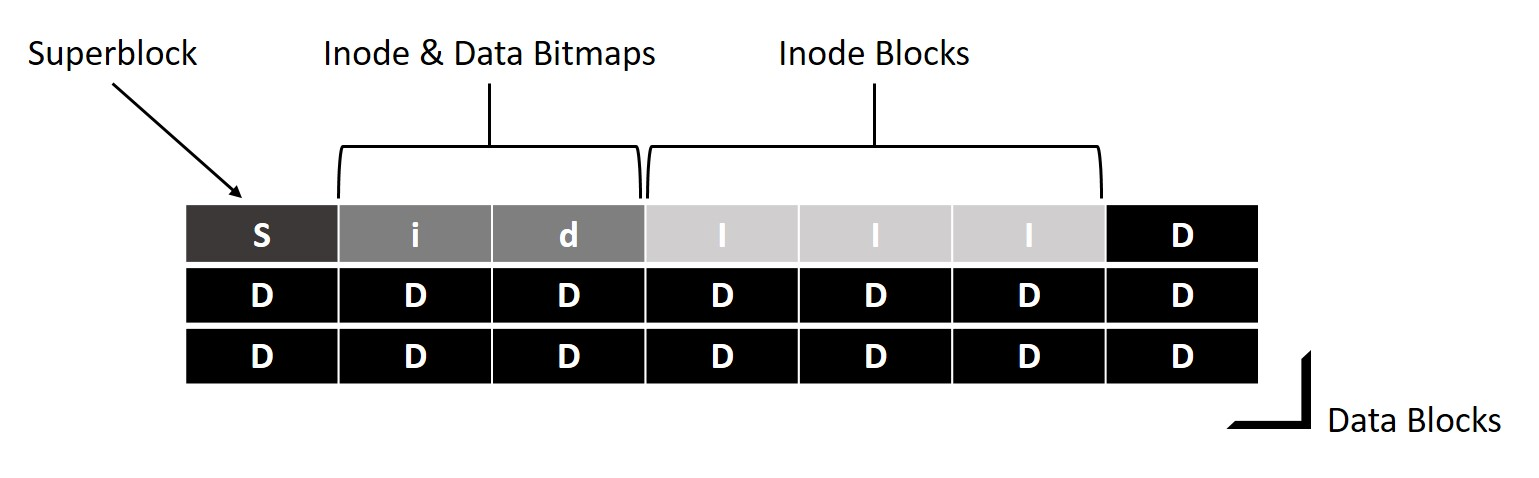
\includegraphics[width=14cm]{img/fs-structure.jpg}}
\caption{Zjednodušená struktura souborového systému založeného na i-uzlech}
\label{fig:fs-structure}
\end{figure}
        
    
    \subsection{Super blok}
 	Super blok je struktura, která popisuje základní informace o souborovém systému.  Označuje například adresu, kde se nachází první i-uzel nebo první datový blok. Dle potřeby je také možné přidat na toto místo jakékoliv jiné informace, jako třeba například velikost jednoho datového bloku.
 	
 	\subsection{Bitmapa}
 	Bitmapa označuje strukturu, která nese informaci o dostupnosti volných i-uzlů a datových bloků. Dle pozice daného bitu se určuje dostupnost položky, kdy hodnota \texttt{0} označuje volnou položku a hodnota \texttt{1} zabranou položku. Při získávání informací z této struktury je vhodné se zamyslet nad efektivitou přístupu, kdy není příliš vhodné načítat použe jednu hodnotu z bitmapy. Ideální je načíst více hodnot než je v daný moment třeba, aby při příštím přístupu k hodnotám byly tyto hodnoty již načtené v operační paměti.
    
    \subsection{I-uzel}
    I-uzel je datová struktura, která v souborovém systému představuje jeden soubor nebo složku. To znamená, že maximální počet i-uzlů představuje maximální možný počet souborů a složek. V této struktuře se typicky nachází informace o tom, kolik dat i-uzel referencuje a jestli představuje o adresář či soubor. 
    
    Pro adresaci dat obsahuje několik přímých ukazatelů na skutečná data souboru či složky. Pokud je soubor objemný, tak se musí použít další ukazatelé na data. Princip vytváření ukazatelů musí být dostatečně flexibilní, aby dokázal referencovat objemná data. Flexibility je dosaženo tak, že i-uzel obsahuje takzvaný \textit{první nepřímý ukazatel} na datový blok, ve kterém jsou v seřazeném pořadí uloženy ukazatele na data souboru. Pokud ani tyto ukazatelé nestačí, tak se využije druhý ukazatel, nazývaný jako \textit{druhý nepřímý ukazatel}, který ukazuje na datový blok, v němž jsou uloženy další ukazatelé typu \textit{první nepřímý ukazatel}. Pokud by ani toto rozšíření nedokázalo pokrýt obsah celého souboru, tak je možné použít další úroveň zanoření, kdy by třetí ukazatel ukazoval na datový blok, jež uchovává odkazy typu \textit{druhý nepřímý ukazatel}.
    
    Jelikož jsou i-uzly v souboru uložené za sebou, tak je možné vynechat identifikační číslo i-uzlu z této struktury a tím ušetřit cenné místo.  
      
\begin{figure}[!ht]
\centering
{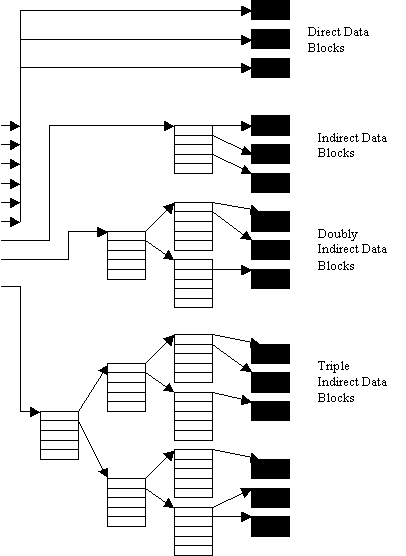
\includegraphics[width=9cm]{img/inodes.png}}
\caption{Adresace dat pomocí inodu}
\label{fig:inodes}
\end{figure}
    
    \newpage
    \subsection{Datový blok}
Datový blok představuje oblast paměti, do které lze zapsat libovolný obsah. Je vyžadováno, aby všechny datové bloky byly stejné velikosti, i přesto, že nějaký blok nemusí být zcela zaplněn. Velikost datových bloků může být libovolná, avšak je třeba dbát na to, že příliš malá velikost datového bloku způsobí, že bude snížena maximální velikost souboru a naopak velká velikost datového bloku bude neefektivní pro složky a malé soubory.

Pokud známe velikost ukazatele na datový blok v souborovém systému, lze pomocí následujícího vzorce spočítat maximální velikost jednoho souboru:

\begin{center}
	$primych\_ukazatelu\times velikost\_bloku + \frac{velikost\_bloku^2}{velikost\_ukazatele} + \frac{velikost\_bloku^3}{velikost\_ukazatele^2} $ 
\end{center}

\subsection{Operace nad souborovým systémem}
	Každý operační systém by měl uživateli poskytovat základní operace pro uschování a manipulaci dat. Mezi nejdůležitější patří následující operace:
	
	\subsubsection{Formátování}
	Tato operace se stará o vytvoření super bloku na základě požadované velikosti souborového systému. Při formátování souborového systému je třeba určit kolik procent diskového místa věnujeme na i-uzly. Jelikož jeden i-uzel představuje jeden soubor, tak pokud očekáváme, že uživatel bude zapisovat spoustu malých souborů, je vhodné přidělit více místa na i-uzly. Pokud je však situace opačná a je předpokládáno méně souborů, které jsou objemné, je vhodnější věnovat místo datovým blokům.
	
	\subsubsection{Přesun souboru v rámci souborového systému}
	Při přesouvání souboru napříč složkami souborového systému se přesouvá pouze ukazatel na soubor (položka složky), nikoliv data souboru či i-uzel.
	
	\subsubsection{Kopírování souboru v rámci souborového systému}
	Kopírování souboru je ve skutečnosti kopírování i-uzlu a dat, jež referencuje, kdy se po duplikaci původního i-uzlu začnou kopírovat data referencovaná původním i-uzlem.

	\subsubsection{Vytvoření nové složky}
	Při vytvoření nové složky, což je v podstatě nový soubor se speciálním formátováním datové části, se musí vytvořit nový i-uzel a do datové části se zapisují položky této složky. Každá složka v souborovém systému ukazuje sama na sebe a nadřazený adresář ve stromové hierarchii.
	
	\subsubsection{Kontrola konzistence}
	Kontrola konzistence je mechanismus, jež odhaluje chyby v struktuře souborového systému. Chyb, které se mohou objevit v souborovém systému, je nespočet.
	 
	 Mezi nejzákladnější chyby, které by měl každý souborový system odhalit, patří chyba, kdy nějaký soubor není referencován žádnou složkou, tudíž k němu nemůže uživatel nikdy přistoupit. Odhalení této chyby může být řešeno velmi jednoduchým způsobem, kdy postupným prohledáváním stromové struktury složek počítáme výskyt souborů. Tento počet výskytů následně porovnáme s počtem zabraných i-uzlů v bitmapě. Pokud tyto dva údaje nejsou shodné, objevili jsme chybu.
	
		Další chybou je například chyba, kdy nějaký i-uzel uvádí jinou velikost referencovaných dat, než velikost dat, které ve skutečnosti referencuje. Avšak tato chyba se ne vždy jednoduše odhaluje, jelikož nelze zcela jednoznačně říct, kolik dat ve skutečnosti i-uzel referencuje. Lze však ověřit, že žádný datový blok by neměl být jedním i-uzlem referencován více než jednou. 
	
	

    \section{Implementace}
    
    	\subsection{Příkazy souborového systému}
		
		\subsubsection{cp}
		Příkaz, který slouží ke kopírování v rámci virtuálního souborového systému, je implementovaný tak, že se nejdříve zduplikuje vybraný i-uzel a poté se začnou kopírovat jednotlivé datové bloky, jež vybraný i-uzel referencuje. Pokud při kopírování dojde místo v souborovém systému, použité datové bloky jsou uvolněny a zduplikovaný i-uzel smazán.
		
		\subsubsection{mv}
		Příkaz, jež přesouvá soubory v rámci virtuálního souborového systému. Přesouvání souboru je implementováno tak, že se pouze smaže záznam o souboru ze složky, ve které se právě přesouvaný soubor nachází, a smazaný záznam se zapíše do cílové složky.
		
		\subsubsection{rm}
		Příkaz, který slouží k mazání souborů ve virtuálním souborovém systému. Smazání je realizováno tak, že se nejdříve uvolní datové bloky, jež soubor referencuje, poté je smazán i-uzel, který soubor představuje a nakonec je smazán záznam o souboru ze složky, ve které se soubor nacházel.

		\subsubsection{mkdir}
		Příkaz, který slouží k vytvoření nové složky ve virtuálním souborovém systému, je implementován tak, že se dle cílové adresy nastaví aktuální i-uzel, ve kterém se přidá nový záznam referencující nový i-uzel, představující vytvořenou složku.
		
		\subsubsection{rmdir}
		Příkaz, který slouží k mazání adresářů ve virtuálním souborovém systému. Smazání je realizováno tak, že se nejdříve uvolní datové bloky, jež složka referencuje, poté je smazán i-uzel, který adresář představuje a nakonec je smazán záznam o souboru ze složky, ve které se složka nacházela. Pro efektivitu smazání položky adresáře je smazání implementováno tak, že místo mazané položky je umístěna poslední položka v seznamu místo toho, aby se celý seznam musel přeuskupovat.
		
		\subsubsection{ls}
		Výpis položek složek je realizován právě tímto příkazem. Příkaz je implementován tak, že se přečtou datové bloky referencované i-uzlem této složky a obsah se převede na seznam záznámů složky, který je následně vypsán.
				
		\subsubsection{cat}
		Výpis obsahu souboru realizován tak, že se nad i-uzlem zavolá průběžné čtení obsahu datových bloků, kdy každý obsah jednotlivého datového bloku je převeden na textový řetězec a následně vypsán. Pokud by se v daném clusteru vyskytoval ukončující znak pro textové řetězce, tak zbytek obsahu clusteru není vypsán.
				
		\subsubsection{cd}
		Přepínání mezi jednotlivými složkami souborového systému je realizováno tak, že se daná adresa rozdělí na názvy jednotlivých složek a dle těchto názvů je v datové části aktivního i-uzlu hledán identifikátor i-uzlu, ke kterému patří aktuálně zpracovávaný název složky.
		
		\subsubsection{pwd}
		Výpis cesty k aktuálním adresáři je realizován právě tímto příkazem, který je implementován tak, že rekurzivně hledá předka aktuální složky, dokud nenarazí na kořenovou složku. Po cestě si pamatuje, které složky navštívil a při nalezení kořenového adresáře vypíše jejich názvy.
		
		\subsubsection{info}
		Výpis informací o vybraném souboru nebo adresáři je realizován právě tímto příkazem, který vypisuje název souboru či adresáře, jeho velikost, identifikátor použitého i-uzlu a seznam adres, kterými jsou referencovány datové bloky.
		
		\subsubsection{incp}
	Pro vytvoření nového souboru se používá právě tento příkaz, který do virtuálního souborového systému nakopíruje vybraný soubor z realného souborového systému. Kopírovaný soubor se čte po blocích o velikosti datového bloku souborového systému. Z těchto dat jsou rázem vytvářeny datové bloky uvnitř souborového systému.
				
		\subsubsection{outcp}
	Pro vykopírování souboru uvnitř virtuálního souborového systému do reálného souborového systému se používá právě tento příkaz, který jednotlivé datové bloky kopírovaného souboru zapisuje do realného souboru.
		
		\subsubsection{load}
	Přečte soubor a jednotlivé řádky interpretuje jako příkazy programu.
		 
		\subsubsection{format}
	Formátování souborového systému je realizováno právě pomocí tohoto příkazu. Nejprve vypočítá počet i-uzlů a datových bloků. Následně určí adresy, kde začínají i-uzly, datové bloky a bitmapa. Tyto údaje zapíše do superbloku, který je následně zapsán do souboru. Nakonec je do souborového systému přidán kořenový adresář.
	
		\subsubsection{check}
	Tento příkaz představuje kontrolu konzistence, která je implementována tak, že se nejdříve rekurzivně prohledá celý strom pro výskyt souborů. Počet všech nalezených souborů se poté porovná s počtem zabraných bitů v bitmapě i-uzlů. Pokud jsou tato čísla odlišná, tak program vypíše, že byla nalezena nekonzistence. Program ještě kontroluje to, zdali udávaná velikost souboru i-uzlem odpovídá tomu, kolik referencuje datových bloků. Při postupném prohledávání adres na datové bloky se hledá adresa  \texttt{0}, která představuje konec ukazatelů, jelikož tato adresa nemůže být platná (na této adrese se nachází začátek superbloku).
		
		\subsubsection{badrm}
	Tento příkaz slouží k vyvolání chyb, které následně může kontrola konzistence odhalit. Chyby jsou vyvolány tak, že se při mazání položky adresáře smaže pouze záznam ve složce, ve kterém se položka nachází. Datové bloky ani i-uzel mazán není. Další chybou, která je úmyslně vyvolána, je ta, že i-uzlu, který představuje položku, se vynuluje první přímý ukazatel na druhý datový blok, čímž poté nemusí sedět udávaná velikost souboru se skutečnou velikostí dat.
		
		
    \subsection{Struktura modulů}
			\subsubsection{aloc.go}
			Tento modul se stará o zápis dat do datových bloků vybraného i-uzlu. Během zápisu dat jsou kontinuálně alokovány clustery, do kterých bude zapisováno. Adresace, funguje tak, že dle pořadí právě zapisovaného clusteru se určí adresa pro zápis dat. Pokud je pořadí menší jak 5, tak se vybere přímý odkaz na data. Další odkazy jsou již nepřímé. Dále je zde implementována funkce \texttt{ReadDataFromInodeFx}, která umožňuje modulární práci se čtenými daty i-uzlu.

			\subsubsection{bitmap.go}
			Poskytuje obecné funkce pro práci s bitmapou. Bitmapa je definována počáteční adresou bitmapy, její délkou v bytech a maximálním počtem bitů, které může obsahovat. Mezi důležitou funkci patří funkce \texttt{FindFreeBitsInBitmap}, která v bitmapě vyhledává volné bity. Při vyhledávání bitů se vyhledá více bitů než je potřeba, které se následně uloží do paměti a později se nemusí znovu přistupovat k souboru.
			\subsubsection{check.go}
			V tomto modulu jsou implementovány funkce pro ověření konzistence souborového systému. Kontola je prováděna dvěmi metodami. První metoda kontroluje, zdali je každý i-uzel referencován nějakým jiným i-uzlem (ověření, že každý soubor se nachází v nějaké složce). Druhá metoda ověřuje to, že udáváná velikost souboru koresponduje s počtem alokovaných datových bloků.

			\subsubsection{cluster.go}
			Pro práci s datovými blokys jsou zde implementovány funkce, které jsou hojně využívány v celém programu. Umožňují například efektivně vyhledat volné ID datového bloku, zapsat do datového bloku adresu nebo například nějaký identifitkátor. Dále poskytuje funkce pro přěvod mezi ID a adresou datového bloku.
			
			\subsubsection{commands.go}
			V tomto modulu jsou implementovány požadované příkazy souborového systému. Funkce v tomto modulu jsou většinou jednoduché a hojně využívají funkce ostatních modulů. Funkce pro interakci se skutečným souborovým systémem jsou složitější, jelikož pracují přímo se soubory.
						
			\subsubsection{dir.go}
			Modul, jež implementuje funkce pro práci s položkami adresáře. Nejsložitejší funkcí je funkce \texttt{AppendDirItem}, která počítá s tím, že může nastat situace, kdy je jedna položka adresáře zapsána do dvou datových bloků. Dále se zde nacházejí funkce pro vyhledávání položek dle ID nebo názvu.
									
			\subsubsection{dir\_traversal.go}
O možnost navigovat mezi jednotlivými adresářemi souborového systému se stará právě tento modul. Poskytuje metody pro rozklíčování cesty na jednotlivé složky a pro změnu aktuálního adresáře. Za zmínku stojí funkce \texttt{VisitDirectoryByPathAndExecute}, která zajistí žmenu aktuálního adresáře na požadovaný, ve kterém zavolá příslušnou funkci, která byla předána parametrem. Nakonec se vrátí do původního adresáře, který byl aktuální před navigací. Většina implementovaných příkazů používá tuto funkci.

\subsubsection{format.go}
Tento modul implementuje metody pro formátování souborového systému a vytvoření superbloku. V rámci formátování se právě vytváří nový superblok a kořenový adresář. Kořenový adresář se vytvoří pouze v případě, že se souborový systém nenachází v testovacím režimu, jelikož testy ověřující funkcionalitu programu počítají s tím, že všechny i-uzly jsou volné.

Při formátování je volné místo rozděleno tak, aby 5\% celkového volného místa zabíraly i-uzly.

\subsubsection{id\_set.go}
Modul, který implementuje datovou strukturu \textit{množina} pro datový typ ID. Tato struktura se využívá při kontrole konzistence, kdy musí být jednotlivé položky adresáře unikátní.

			\subsubsection{inode.go}
Pro práci s i-uzly slouží právě tento modul, který poskytuje funkce pro vyhledávání volného i-uzlu, vytvoření nového i-uzlu a pro převod mezi adresami a identifikátory i-uzlů.

			\subsubsection{myfilesystem.go}
Definuje strukturu, jež představuje souborový systém. Dále poskytuje funkci \texttt{Load}, která se pokusí načíst souborový systém ze souboru. 

			\subsubsection{structs.go}
Definice základních struktur, které se používají napříč souborovým systémem. Nachází se zde například definice struktury reprezentující i-uzel nebo datový blok.

			\subsubsection{tests}
V tomto modulu se nachází 47 testů, které ověřují funkcionalitu souborového systému.


			
        \section{Překlad a spuštění aplikace}
        Pro překlad a spuštění aplikace je vyžadován následující software:
        \begin{itemize}
                \item go1.13.1 či novější
        \end{itemize}
        V kořenu projektu přeložte aplikaci pomocí příkazu \texttt{go build -o kral\_zos\_sp}. Poté aplikaci spusťte příkazem \texttt{./kral\_zos\_sp}, kdy první parametr, označující soubor použitý pro souborový systém, je nepovinný (použije se výchozí název souboru \texttt{myfs}).


    \section{Závěr}
    V rámci této semestrální práce byl vytvořen program v jazyce GoLang, který simuluje souborový systém. Souborový systém je simulován tak, že se jako médium používá soubor v reálném souborovém systému.
    
    Byly implementovány všechny požadované příkazy, která byly uvedeny v zadání semestrální práce. Vývoj probíhal tak, že na veškeré základní funkce souborového systému byly ihned psané jednotkové testy, čímž byla ověřena funkcionalita těchto funkcí. Ve výsledku toto zapříčinilo to, že kód testů je stejně dlouhý jako kód samotného programu. Následná implementace požadovaných příkazů poté byla velmi jednoduchá a bezproblémová, protože základní funkcionalita souborového systému byla velmi spolehlivá a ověřená 47 testy. Díky tomu se volba jazyka GoLang ukázala jako velmi vhodná, jelikož v základní knihovně, narozdíl například od jazyka C, poskytuje podporu pro psaní testů.
    
    Program by mohl následně být rozšířen o možnost kopírovat celé složky včetně jejich obsahu, což v aktuální verzi neumožňuje.

    


%obrazek
%\begin{figure}[!ht]
%\centering
%{\includegraphics[width=12cm]{img/poly-example.jpeg}}
%\caption{Zjednodušené UML aplikace (pouze balíčky)}
%\label{fig:photo}
%\end{figure}

	\listoffigures
	

\end{document}    